\section{Simulation}

\subsection{Delay-Modell}
Das Transport-Modell (1) verzögert in jedem Fall um die mit \textit{after} definierte Zeit.\\
Das Inertial-Modell (2) muss länger als die mit \textit{after} definierte Zeit sein, ansonsten wird dieser verschluckt.
\begin{lstlisting}
	-- (1)
y <= transport a or b after 10 ns;
	-- (2), auch inertial
y <= a or b after 10 ns;
\end{lstlisting}

\begin{center}
	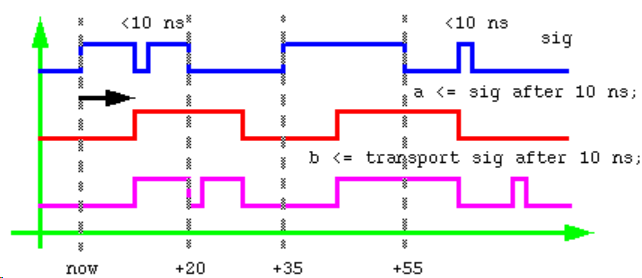
\includegraphics[width=0.8\columnwidth]{Images/transport_example}
\end{center}



\subsection{Testbanche}
\begin{lstlisting}
library ieee;

entity glue_logic_tb is
-- meist leer
end;

architecture tb of glue_logic_tb is
	component glue_logic
		port(in0 : in  bit);
	end component glue_logic;
	
	for all : glue_logic use entity work.glue_logic(behavioral);

	signal s0 : bit;
	
	constant SIM_CYC : time := 100 ns;
begin

dut : component glue_logic port map(in0 => tb_in0);

clock_p : process
begin
	clk <= '1'; wait for (SIM_CYC/2);
	clk <= '0'; wait for (SIM_CYC/2);
end process;

s0 <= '0', 
      '1' after 20ns,
      '0' after 10ns,
      '1' after 60ns;
      
response : process 
begin
  wait for 80 ns;
  assert (s0 <> '0') report "Error Messgage" warning;
  wait;
end process;

end tb;
\end{lstlisting}
